\section{Experimental setup of Pockels effect}
The experimental setup



Using the definition $n = \sqrt{\eps}$, we can calculate $\eps_x$:
\begin{align}
    \eps_1 &= n_1^2 = 2.408 \\
    \eps_3 &= n_3^2 = 2.182 \\
    \eps_x &= \frac{2 \eps_1 \eps_3}{\epsn \left( \eps_1 + \eps_3\right)} = 2.289
\end{align}


\subsection{Properties of He-Ne-Laser}
In this experimental setup we use a helium-neon laser, which is one of the most popular lasers.
The inherent gain medium consists of a 10-1 ratio mixture of helium and neon 
at a pressure of 10mbar. The laser
was developed in 1961 as first \textbf{continuous wave}-laser. It has been used since then to
study general properties of lasers and of coherent light in general, which originates from
the neonatoms being stimulated by the helium. Nowadays helium-neon lasers are more and more
replaced and substituted by the more compact and inexpensive laser diode.
The functional principle is as following: A external induced discharge causes the helium atomes
to shift into a higher, persistent energy level. From this time the neonatomes can be stimulated
continuosly with a high efficiency and cause thus an inversion of the higher energy levels.
Without helium we would not see the higher excited states. The pump source of the laser
is in general realized by a high voltage electrical discharge coming from an anode and
cathode with the gas in between, within the tube. Since the intensity is connected to the
pressure it is possible to increase the length of the tube in order to amplify the beam, which
has other disadvantages, for instance the appeareance of other unwanted lines.
The electromagnetic field $E(\rho = \sqrt{x^2 + y^2}, y)$ with Amplitude $E_0$ 
generated by the laser can be treated approximately as a gaussian
beam~\cite{boyd2003nonlinear}, which follows the following equation:
\begin{equation}
    E(\rho,z) = \frac{E_0 w_0}{w(z)} \mathrm{Exp} \left[  
        \frac{ik\rho^2}{2R(z)} + i\phi(x) - \left( \frac{\rho}{w(z)} \right)^2    \right]
\end{equation}
Where we introduced the 1/e radious of the field distribution
\begin{align}
    w(z) = w_0 \sqrt{ 1 +\left (\frac{\lambda z}{\pi w_0^2} \right )^2}
\end{align}
and the radius of the curvature of the optical wavefront with
\begin{equation}
    R(z) = z \left[ 1 + \left( \frac{\pi w_0^2}{\lambda z} \right)^2 \right]
\end{equation}
and the spatial variation of the phase of the wave
\begin{equation}
    \phi(z) = - \mathrm{Arctan} \left( \frac{\lambda z}{\pi w_0^2} \right) 
\end{equation}

\begin{SCfigure}
    \begin{centering}
        \caption{The inversion of the helium-neon laser~\cite{christian2003gerthsen}. 
            As result of the electronscattering the
    heliumatoms are shifted into persistent states, from which they transmit their energy by
    interaction to the neon. The highest laser activity is realized
    through the shift of 3s to 2p states ($633nm$) but other lines are possible as well,
    for instance from 3s to 3p ($3.39 \mu m$) or from 2s to 2p ($1.15\mu m$). The mechanism
    producing this population inversion and the light amplification in the plasma is due
    to the inelastic scattering of the electrons with ground state helium atoms in the gas
    mixture.}
        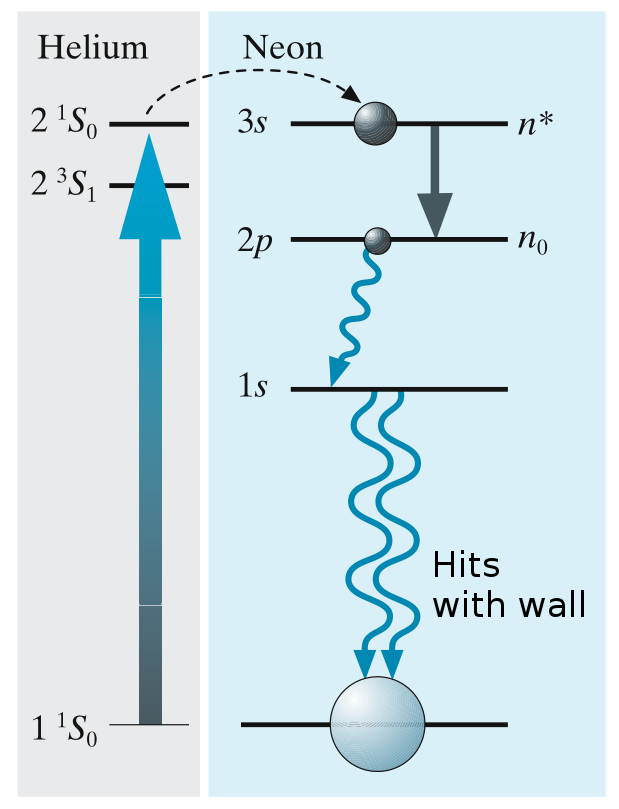
\includegraphics[width=8cm]{figures/helium-neon-laser}
        \label{fig:integral}
    \end{centering}
\end{SCfigure}

\begin{SCfigure}
    \begin{centering}
    \caption{Different aspects of the gaussian nature of the laser beam~\cite{boyd2003nonlinear}.
        (a) Field amplitude distribution of a gaussian laser beam. (b) Variation of the beam
        radius $w$ and wavefront radius of curvature R with position $z$.
        (c) Relation between the beam waist radius and the confocal parameter $b$. }
        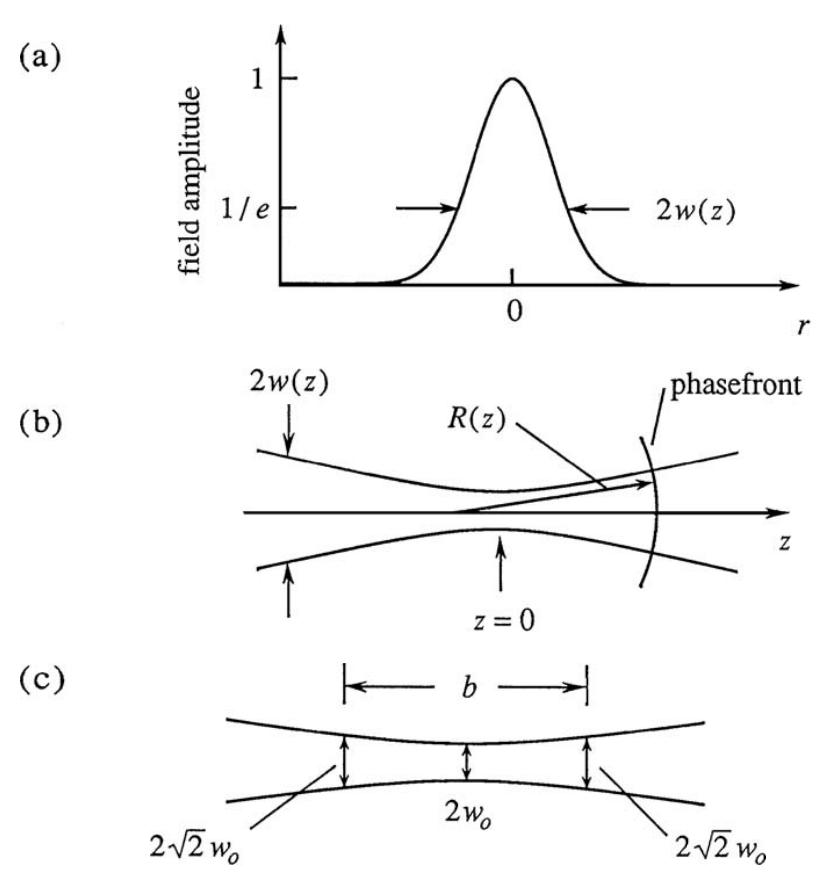
\includegraphics[width=10cm]{figures/gaussian}
        \label{fig:integral}
    \end{centering}
\end{SCfigure}
The beam waist radius $w_{0}$ can be calculated in terms of the Power $P$, which we can retrieve
by integrating:
\begin{equation}
    P = n \epsilon_0 c \pi w_0^2 |E_0|^2
\end{equation}
Unfortunatelly in our experimental setup it was neither possible to modificate the position of
the laser nor to adjust the setup in a way that we could have measured the specifications of 
the laser, so it is not possible for us to include dispersion or diffraction phenomena originating
from the gaussian nature of the beam into our considerations regarding to the analysis of the 
experiment. We added some notes in the chapter~\ref{sec:laser} ``
Further investigations regarding the laser''.




